\section{Introdução}

\subsection{Padrões}
    \begin{frame}[fragile]{Definição de Padrões}
        \begin{figure}[H]
        \begin{center}
            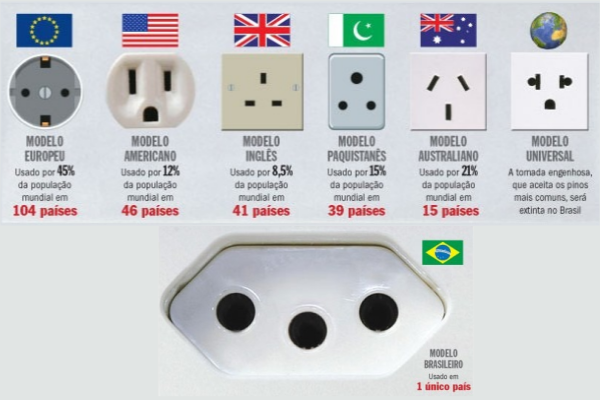
\includegraphics[scale=0.50]{images/padroes.png}
        \end{center}
        \end{figure}

        São perceptíveis \textbf{regularidades} que repetem-se de maneira
        \textbf{previsível} no  mundo ou em um artefato produzido pelo homem.
    \end{frame}

    \begin{frame}[fragile]{Os Padrões no Mundo}
        \begin{figure}[H]
        \begin{center}
            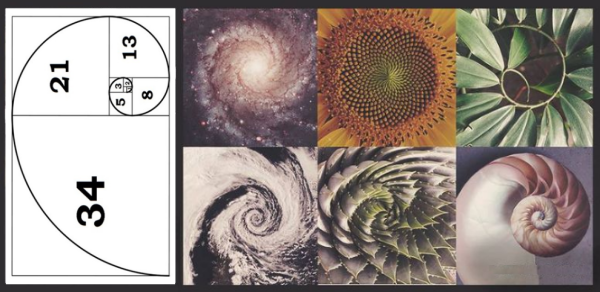
\includegraphics[scale=0.60]{images/padroes_mundo.png}
        \end{center}
        \end{figure}

        Mendes (2007) explica, em seu estudo sobre a matemática na
        \textbf{natureza}, a ocorrência da \textbf{sequência} de
        \textbf{Fibonacci} na Natureza é tão frequente que é difícil acreditar
        que é acidental.
    \end{frame}

    \begin{frame}[fragile]{Os Padrões nos Artefatos}
        \begin{figure}[H]
        \begin{center}
            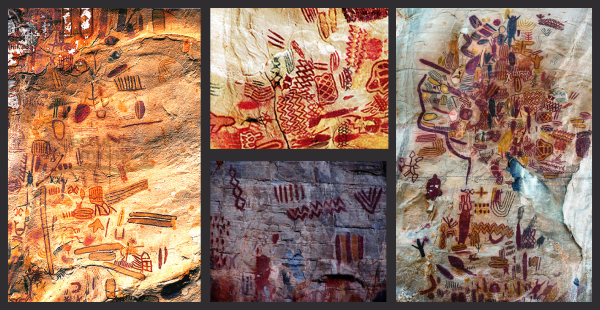
\includegraphics[scale=0.60]{images/arte_rupestre.png}
        \end{center}
        \end{figure}

        Ribeiro, L. (2007) em seu trabalho, classifica os estilos de pinturas
        rupestres do norte mineiro e sudoeste baiano.
    \end{frame}

\subsection{Aprendizado de Máquina}
    \begin{frame}[fragile]{Aprendizado de Máquina}
        \begin{figure}[H]
        \begin{center}
            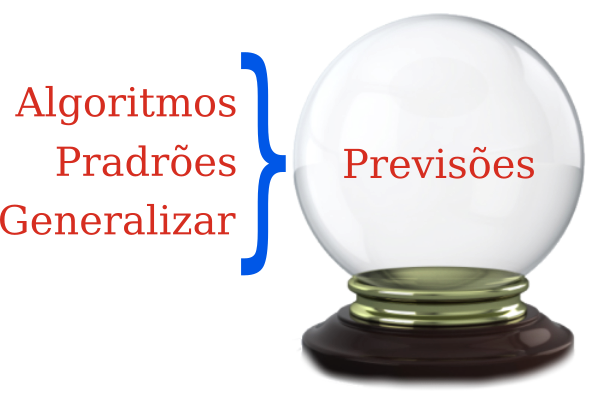
\includegraphics[scale=0.50]{images/previsao.png}
        \end{center}
        \end{figure}

  Aprendizado de máquina é uma subárea da inteligência artificial, ela permite
que computadores tomem decisões com ajuda de algoritmos que reconhece
padrões em conjuntos de dados e se tornam capazes de fazer previsões.
  \end{frame}

\subsection{Problema de Pesquisa}
  \begin{frame}[fragile]{Problema de Pesquisa}
  \end{frame}